%% mapping.tex
%% Author: Leighton Pritchard
%% Copyright: James Hutton Institute
%% These slides give a short, high-level account of read mapping in 
%% sequence assembly

% SUBSECTION: Short-Read Sequence Alignment
% A short account of Read Mapping
\subsection{Short-Read Sequence Alignment}

% Graphical example of OLC
\begin{frame}
  \frametitle{Why map reads?\footnote{\tiny{\href{http://dx.doi.org/10.1038/nbt0509-455}{Trapnell \textit{et al}. (2009) \textit{Nat. Biotech.} \textbf{27}:455-457 doi:10.1038/nbt0509-455}}}}
  ``Resequencing'' an organism (really: a close relative, looking for SNPs/indels)\\
  To see where reads map on an assembled genome\\
  \begin{itemize}
    \item Is coverage even? (can indicate repeats)
    \item Are there SNPs/indels? (heterogeneous population)
    \item Assembly problems?
  \end{itemize}  
\end{frame}

% An overview of short-read sequence alignment
\begin{frame}
  \frametitle{Short-Read Sequence Alignment\footnote{\tiny{\href{http://dx.doi.org/10.1038/nbt0509-455}{Trapnell \textit{et al}. (2009) \textit{Nat. Biotech.} \textbf{27}:455-457 doi:10.1038/nbt0509-455}}}}
  An embarrassment of tools (over 60 listed on \href{http://en.wikipedia.org/wiki/List_of_sequence_alignment_software}{Wikipedia})\\
  Main approaches:
  \begin{itemize}
    \item \textbf{Alignment}: Smith-Waterman mathematically guaranteed to be the best alignment available (e.g. BFAST, MOSAIK);  approximation to S-W (e.g. BLAST); ungapped or gapped alignment (e.g. MAQ, FAST, mrFAST, SOAP). Can be slow.
    \item \textbf{Burrows-Wheeler Transform}: Makes permanent reusable index of the genome (e.g. Bowtie, BWA), can be extended to consider sequence probability (e.g. BWA-PSSM). Can be very fast.
  \end{itemize}
  Other tools may employ different algorithms, some designed to be parallelised on GPUs/FPGAs (e.g. NextGenMap, XpressAlign)
\end{frame}

% Graphical example of OLC
\begin{frame}
  \frametitle{Visualising Read Mapping}
  Several tools are available, e.g. Tablet\footnote{\tiny{\href{http://dx.doi.org/10.1093/bib/bbs012}{Milne \textit{et al}. (2013) \textit{Brief. Bioinf.} \textbf{14}:193-202 doi:10.1093/bib/bbs012}}}
  \begin{center}
    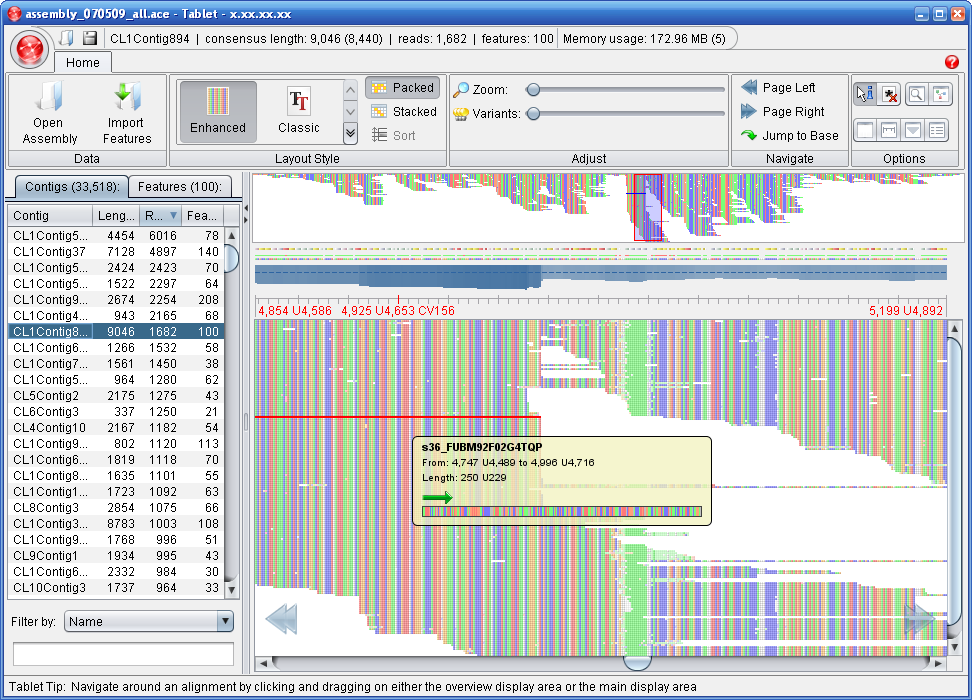
\includegraphics[height=0.65\textheight]{images/tablet1}
  \end{center}  
\end{frame}
